
%%%
% Any line that begins with a percent symbol is a comment. To compile
% this document and view the output:
%
% Run Latex
% Run Bibtex
% Then run Latex twice.
%
% This should produce the output PDF file named main.pdf
%%%

% This defines the style to use for this document.
% Do not modify.
\documentclass[letterpaper]{article}

% The following are akin to "import" statements in Python or Java -
% these import useful commands into the document for you to use.  You
% don't have to modify any of these lines. The AAAI package formats
% this document in the style of submissions to the American
% Association for Artificial Intelligence conference, one of the top
% AI conferences in the world. You will find that many academic
% publications in AI use this format.
\usepackage{aaai} 
\usepackage{times} 
\usepackage{helvet} 
\usepackage{courier} 
\setlength{\pdfpagewidth}{8.5in} 
\setlength{\pdfpageheight}{11in} 
\usepackage{amsmath}
\usepackage{amsthm}
\usepackage{graphicx}
\usepackage{graphics}
\usepackage{moreverb}
\usepackage{subfigure}
\usepackage{epsfig}
\usepackage{txfonts}
\usepackage{algpseudocode}
\usepackage{multirow, multicol}
\usepackage{url}
\usepackage{tablefootnote}
\usepackage{color}

\setcounter{secnumdepth}{1}
\nocopyright

% Fill in your paper title, names and emails below
% The "\\" is used to break lines. The \url command
% is useful for typesetting URLs and email addresses (it uses the
% Courier font).
\title{Handwritten Digit Recognition Using Multilayered Learning and Elastic Matching}
 \author{Mutian Chen \and Ryland Wheliss\\
 \url{{kychen, rywheliss}@davidson.edu}\\
 Davidson College\\
 Davidson, NC 28035\\
 U.S.A.}

% This is the "true" start of the document. All the text in your
% write-up should be placed within the \begin{document} and
% \end{document} decorators.
\begin{document}

\maketitle % formats the title nicely, do not modify

% While at this point you could just begin your write-up, often, it's
% useful to write each section of your write-up in a separate tex
% file (not unlike the modular decomposition you do for code you
% write). These \input commands insert the contents of the
% specified tex files in the order specified. Every write-up you
% submit must contain the following sections, in the shown order. Open
% each of the indicated tex files to understand what goes in each
% section, as well as for more TeX tips.

% Place the contents of your abstract between the
% \begin{abstract} and \end{abstract} decorators.

\begin{abstract}

The abstract should be between four and seven sentences long. Introduce the
problem you are studying. Describe what you did. Summarize your results --- what
did you discover, what is the main take-away message? Basically, you're trying 
to sell your paper to the reader, so be brief and to the point. \textbf{Do \emph{not}
include any citations in the abstract.}

% The \textbf{} command makes the specified text bold. The \emph{} or
% \textit{} command are used to italicize text. In general, text is never
% underlined.

% DON'T FORGET TO MATCH EACH OPEN BRACE WITH A CLOSING BRACE!
\end{abstract}



% The \section{} command formats and sets the title of this
% section. We'll deal with labels later.
\section{Introduction}
\label{sec:intro}

For this assignment we were given a MNIST dataset which consisted of 60,000
handwritten letters that each were converted into 28 x 28 set of
pixels displaying the color of each pixel. There was then a label for
each letter that we were then asked to predict for a test set. We
investigated different classifiers and looked at many resources to
determine what the greatest predictors were.\\ 

We investigated the use of MultiLayered Perceptron which was described
in the paper “One Against One” or “One Against All”: Which One is
Better for Handwriting Recognition with SVMs?, from there
we discovered the scikit learn had the same classifier\cite{milgram}. 


% Citations: As you can see above, you create a citation by using the
% \cite{} command. Inside the braces, you provide a "key" that is
% uniue to the paper/book/resource you are citing. How do you
% associate a key with a specific paper? You do so in a separate bib
% file --- for this document, the bib file is called
% project1.bib. Open that file to continue reading...

% Note that merely hitting the "return" key will not start a new line
% in LaTeX. To break a line, you need to end it with \\. To begin a 
% new paragraph, end a line with \\, leave a blank
% line, and then start the next line (like in this example).




\section{Background}
\label{sec:background}

We investigated into the course of multi-layer perceptron. This is a
Neural Network regression classifier that includes a hidden layer
where the input is transformed into a more seperable layer. Many
hidden layers can be added to the model and we used two different
transformations to create the hidden data. The first is the identity
which is a no-operation activation. It just returns the same out put
as was inputed or $f(x)=x$. The second transformation we used was
described in the paper tilte,
and transformed the input into a rectified linear unit function.\cite{milgram} This
transformation returns $f(x)=max(0,x)$ and was used in the paper as a
baseline but we had not fully understood their further studys and so
this became one of our better classifiers. \\

Looking more into the multi-layer transformations we came across
Reading Checks with Multilayer Graph Transformer Netwroks
\cite{cun}. This paper went even more indepth into multilayer neural
net training. It spoke a lot about its use in efficiently computing
the gradients of the function as well as going into the mathematical
side of the hidden layers or as they called it, the convolutional
layer. We used some of their research and testing in Gradient Based
Learning to determine the number of layers to use as well as which
classifiers not to use. \\






\section{Experiments}
\label{sec:expts}
It should be noted that in the original data set if every pixel grey scale value were to be used as a feature to train for the model might result in a huge set of features. Having such set of features may cause a commnon phenomena known as "the curse of dimensionality", which implicates that the increase in the dimensional space resulted from the increase in the number of features might dilute the statisical significance of the final result.\cite{bellman}
That being said, in order to reduce the complexity of the final model in the hope of avoiding overfitting problems, a feature selection process was implemented for the experiments.\cite{hall}
\subsection{Feature Selections}
\label{feature}
According to Hall, feature selection process consists of the following steps:
\begin{itemize}
	\item Starting point
	\item Search orgnization
	\item Evaluation strategy
	\item Stopping criterion

\end{itemize}
As introduced in the "Data Preparation" section, after some inspections through the data sets, it was observed that some pixels' grey scale values stayed the same all the time. Those points generally tend to have no significant impacs on the predictions according to the low-variance rule. Thus, those features could be the starting points. For this purpose,the backward elemination method was adpoted to reduce the number of features.\cite{hall}
The evaluation strategy is basically reducing the features that have zero variance one by one  using the variance-based feature selection method implemented in the scikit-learn library. This process was repeated until the results showed significant decline in the models generated by the learning algorithms. For the purpose of determining the optimal set of features, the SVM algorithm was implemented because of its short running time.

\subsection{Classifiers}
\label{class}
For this particular classification problem, several models were implemented and tested out. Here
\paragraph{Super Vector Machines}
SVM serves as the baseline model for the experiments due to its simplistic nature. It is also used for finding the optimal set of features.
\paragraph{Multi-layered Perceptron}



\section{Results}
\label{sec:results}

Present the results of your experiments. Simply presenting the data is
insufficient! You need to analyze your results. What did you discover?
What is interesting about your results? Were the results what you
expected? Use appropriate visualizations. Prefer graphs and charts to
tables as they are easier to read (though tables are often more
compact, and can be a better choice if you're squeezed for space).

\subsection{Embedding Pictures}
\label{subsec:pics}

See the source code (\texttt{results.tex}) for instructions on how to
insert figures (like figure~\ref{fig:tex}) or plots into your
document.

% Note that TeX has a mind of its own when it comes to placing images
% in documents - where a figure appears in the PDF document will often
% be quite different from where it appears in the source code. This is
% a feature, not a bug - it enables LaTeX to produce layouts that
% "flow" better. It only takes a few lines to insert a figure into
% your write-up - I recommend using PNG, JPG or PDF images
% (incidentally, programs like Excel and Matlab will allow you to save
% any plots or figures you generate in those formats). The \figure{}
% command is used to create a new figure.
\begin{figure}[htb]

  \centering  % centers the image in the column

  % replace the second argument below with your filename. I like to
  % place all my figures in a sub-directory to keep things organized
  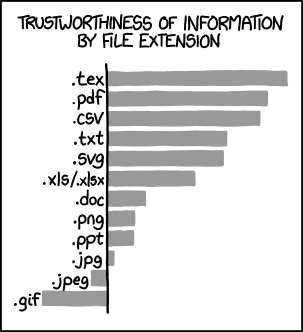
\includegraphics[width=0.47\textwidth]{figs/file_extensions.png}

  % *Every* figure should have a descriptive caption.
  \caption{On the trustworthiness of \LaTeX. Image courtesy of \texttt{xkcd}.}

  % The label is a handle you create so that you can refer to this
  % figure (using the \ref{} command) from other parts of your
  % document. LaTeX automatically renumbers figures and updates
  % references when you recompile, so you should do it this way rather
  % than hard-coding in references. Notice that I've also been
  % creating labels for the various sections in the document; I could
  % use \ref{} command to refer to those sections using their labels
  % too.
  \label{fig:tex}

\end{figure}

\subsection{Creating Tables}
\label{subsec:tables}

Again, refer to \texttt{results.tex} to learn how to create simple
tables (like table~\ref{tab:example}).
\begin{figure}[htb]
  \centering % centers the entire table

  % The following line sets the parameters of the table: we'll have
  % three columns (one per 'c'), each
  % column will be centered (hence the 'c'; 'l' or 'r' will left or
  % right justify the column) and the columns
  % will have lines between them (that's the purpose of the |s between
  % the 'c's).
  \begin{tabular}{|c|c|c|} 
    \hline \hline % draws two horizontal lines at the top of the table
    Column 1 & Column 2 & Column 3 \\ % separate column contents using the &
    \hline % line after the column headers
    $1$ & $3.1$ & $2.7$ \\
    $42$ & $-1$ & $1729$\\
    \hline \hline
  \end{tabular}

  % As with figures, *every* table should have a descriptive caption
  % and a label for ease of reference.
  \caption{An example table.}
  \label{tab:example}

\end{figure}



\section{Conclusions}
\label{sec:concl}

In this section, briefly summarize your paper --- what problem did you
start out to study, and what did you find? What is the key result /
take-away message? It's also traditional to suggest one or two avenues
for further work, but this is optional.


\section{Contributions}
\label{sec:contrib}

Mutian wrote the SVD classifier as well as the feature selection
code. Ryland wrote the MLP classifier code as well as investigated
more into the testing and training sets. Ryland wrote the
Introduction, and bund Information, the Citations, the
Contributions, the Acknowledgements and the experiments. Mutian wrote part of the experiments,  results and the conclusion. Mutian was
also big into researching what other people had done while Ryland
interpreted those readings to work as classifiers.

\section{Acknowledgements}
\label{sec:ack}

We would like to thank Dr. Ramanujan for answering some of our questions
throughout the process as well as some of our classmates who helped in tough
points. 


% This creates the references section. Open the project1.bib file to
% see how to organize your references.
\bibliography{project1}
\bibliographystyle{aaai} % sets citation and bib style, do not modify

\end{document}
